\chapter{Problem Statement}

We are going to develop a website for ``Krushi"
\section{Objective}
The objectives of the proposed system will be as follows:
\begin{enumerate}
\item  Developed a web-based platform that will assist farmers in their agricultural activities. 
\item Implemented a plant disease detection module that will identify crop diseases from leaf images using machine learning techniques. 
\item  To develop a soil analysis module that will provide crop based on soil parameters. 
\item Designed an AI-powered chatbot that will provide real-time agricultural guidance and query support. 
\item To integrate an online agricultural marketplace for purchasing seeds, fertilizers, and farming tools. 
\item Promote digital agriculture and support farmers through technology-based solutions.
\end{enumerate}
\newpage
\section{Scope}
\begin{enumerate}
\item The Krushi system will provide a unified digital platform that will support farmers by offering
plant disease detection, soil analysis, chatbot assistance, and an online agricultural shop in a
single integrated system. 
\item The platform will allow farmers to upload leaf images for disease detection, enter soil
parameters for fertility assessment, and receive crop and fertilizer recommendations based on
system analysis. 
\item  The chatbot module will be designed to provide instant agricultural guidance, answer queries, and support farmers with basic farming information and recommendations. 
\item The online shop module will enable farmers to browse and purchase agricultural products such
as seeds, fertilizers, tools, and equipment through a secure payment and transaction
management system. 
\item The system will support user authentication, record management, and admin-based product
management to ensure secure, organized, and scalable platform operations. 
\item The scope of the system will primarily focus on assisting farmers at a digital level by improving
decision-making, awareness, and accessibility to agricultural resources.
\end{enumerate}
\newpage
\section{Design Overview }
\subsection{Data flow diagrams}
\begin{enumerate}
  \item \textbf{LEVEL 0}

\begin{figure}[H]
 \centering
  % Requires \usepackage{graphicx}
 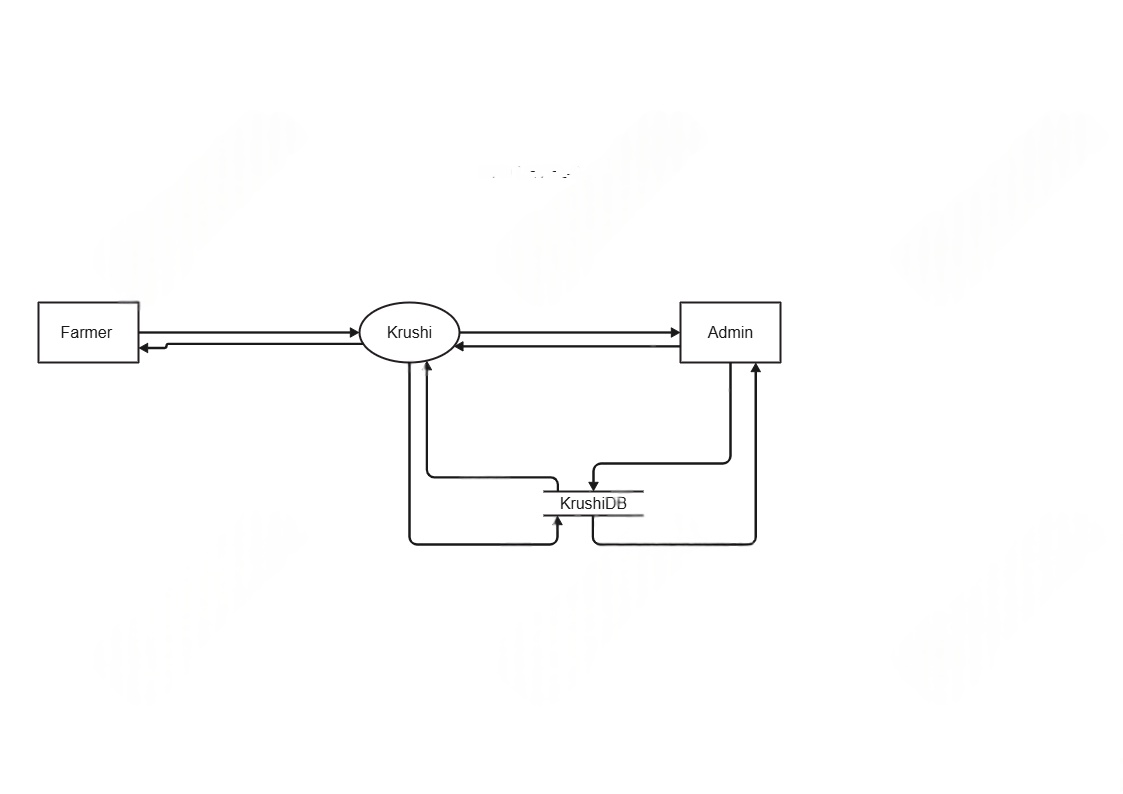
\includegraphics[scale=0.5]{project/images/image/dfd0}
  \caption{Level 0 Data flow diagram}\label{Level 0 DFD}
\end{figure}
\newpage
  \item  \textbf{LEVEL 1}
  \begin{figure}[H]
 \centering
  % Requires \usepackage{graphicx}
  % Requires \usepackage{graphicx}
 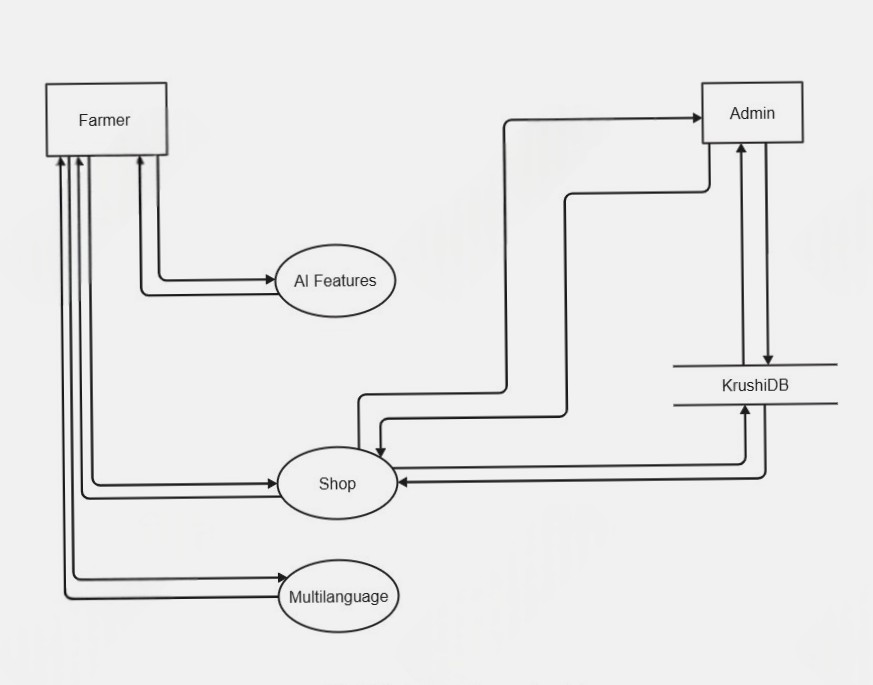
\includegraphics[scale=0.69]{project/images/image/dfd1}
  \caption{Level 1 Data Flow Diagram }\label{Level 1 DFD}
\end{figure}
\newpage
\item \textbf{LEVEL 2}
\begin{figure}[H]
\centering
  % Requires \usepackage{graphicx}
 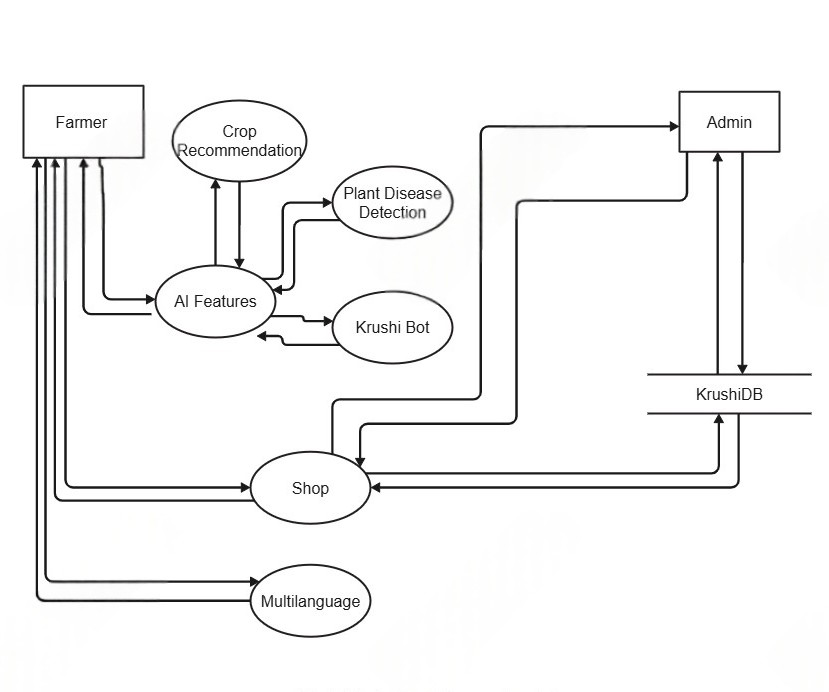
\includegraphics[scale=0.86]{project/images/image/dfd2}
  \caption{Level 2 Dataflow Diagram}\label{Level 2 DFD}
\end{figure}
\end{enumerate}
\newpage
\subsection{UML Diagram}
\begin{enumerate}
   \item \textbf{Use case Diagram}
   \begin{figure}[H]
 \centering
  % Requires \usepackage{graphicx}
 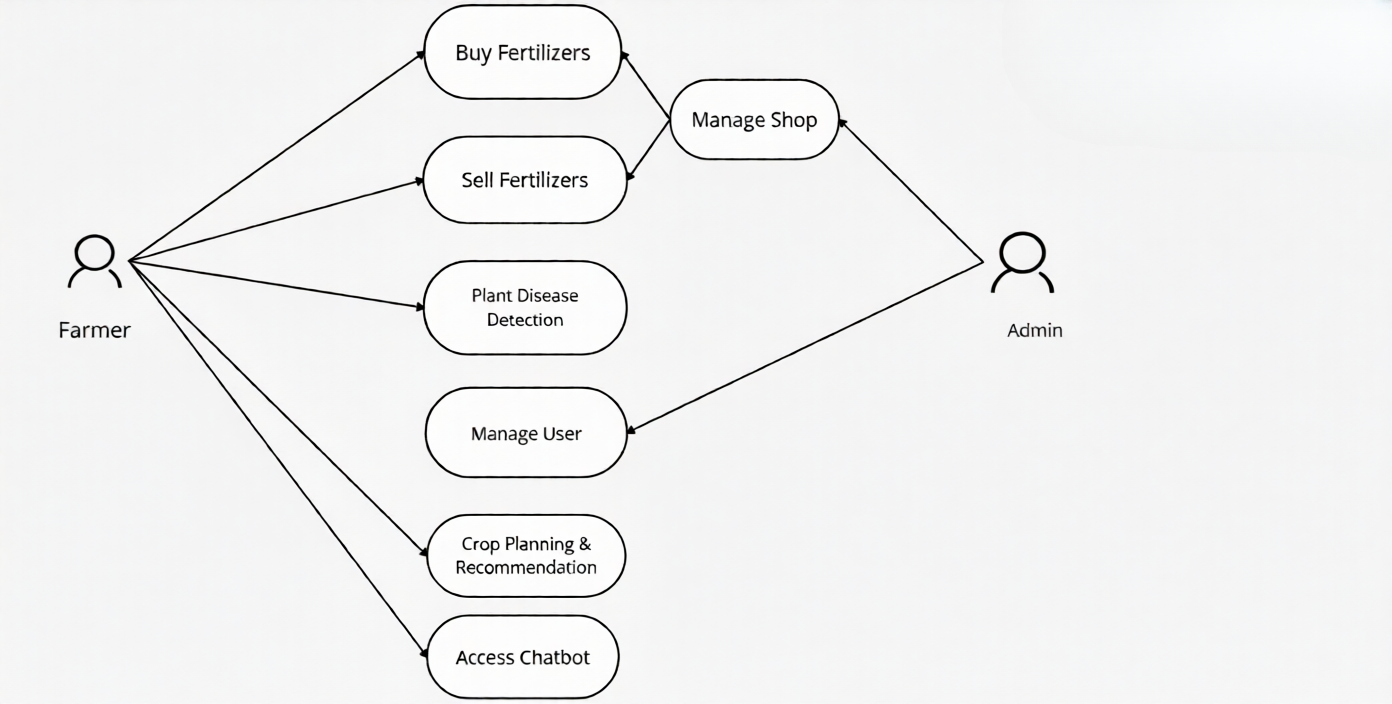
\includegraphics[scale=0.4]{project/images/image/usecase}
  \caption{Use case Diagram}\label{Use case Diagram}
\end{figure}
\newpage
  \item \textbf{Sequence Diagram}
   \begin{figure}[H]
 \centering
  % Requires \usepackage{graphicx}
 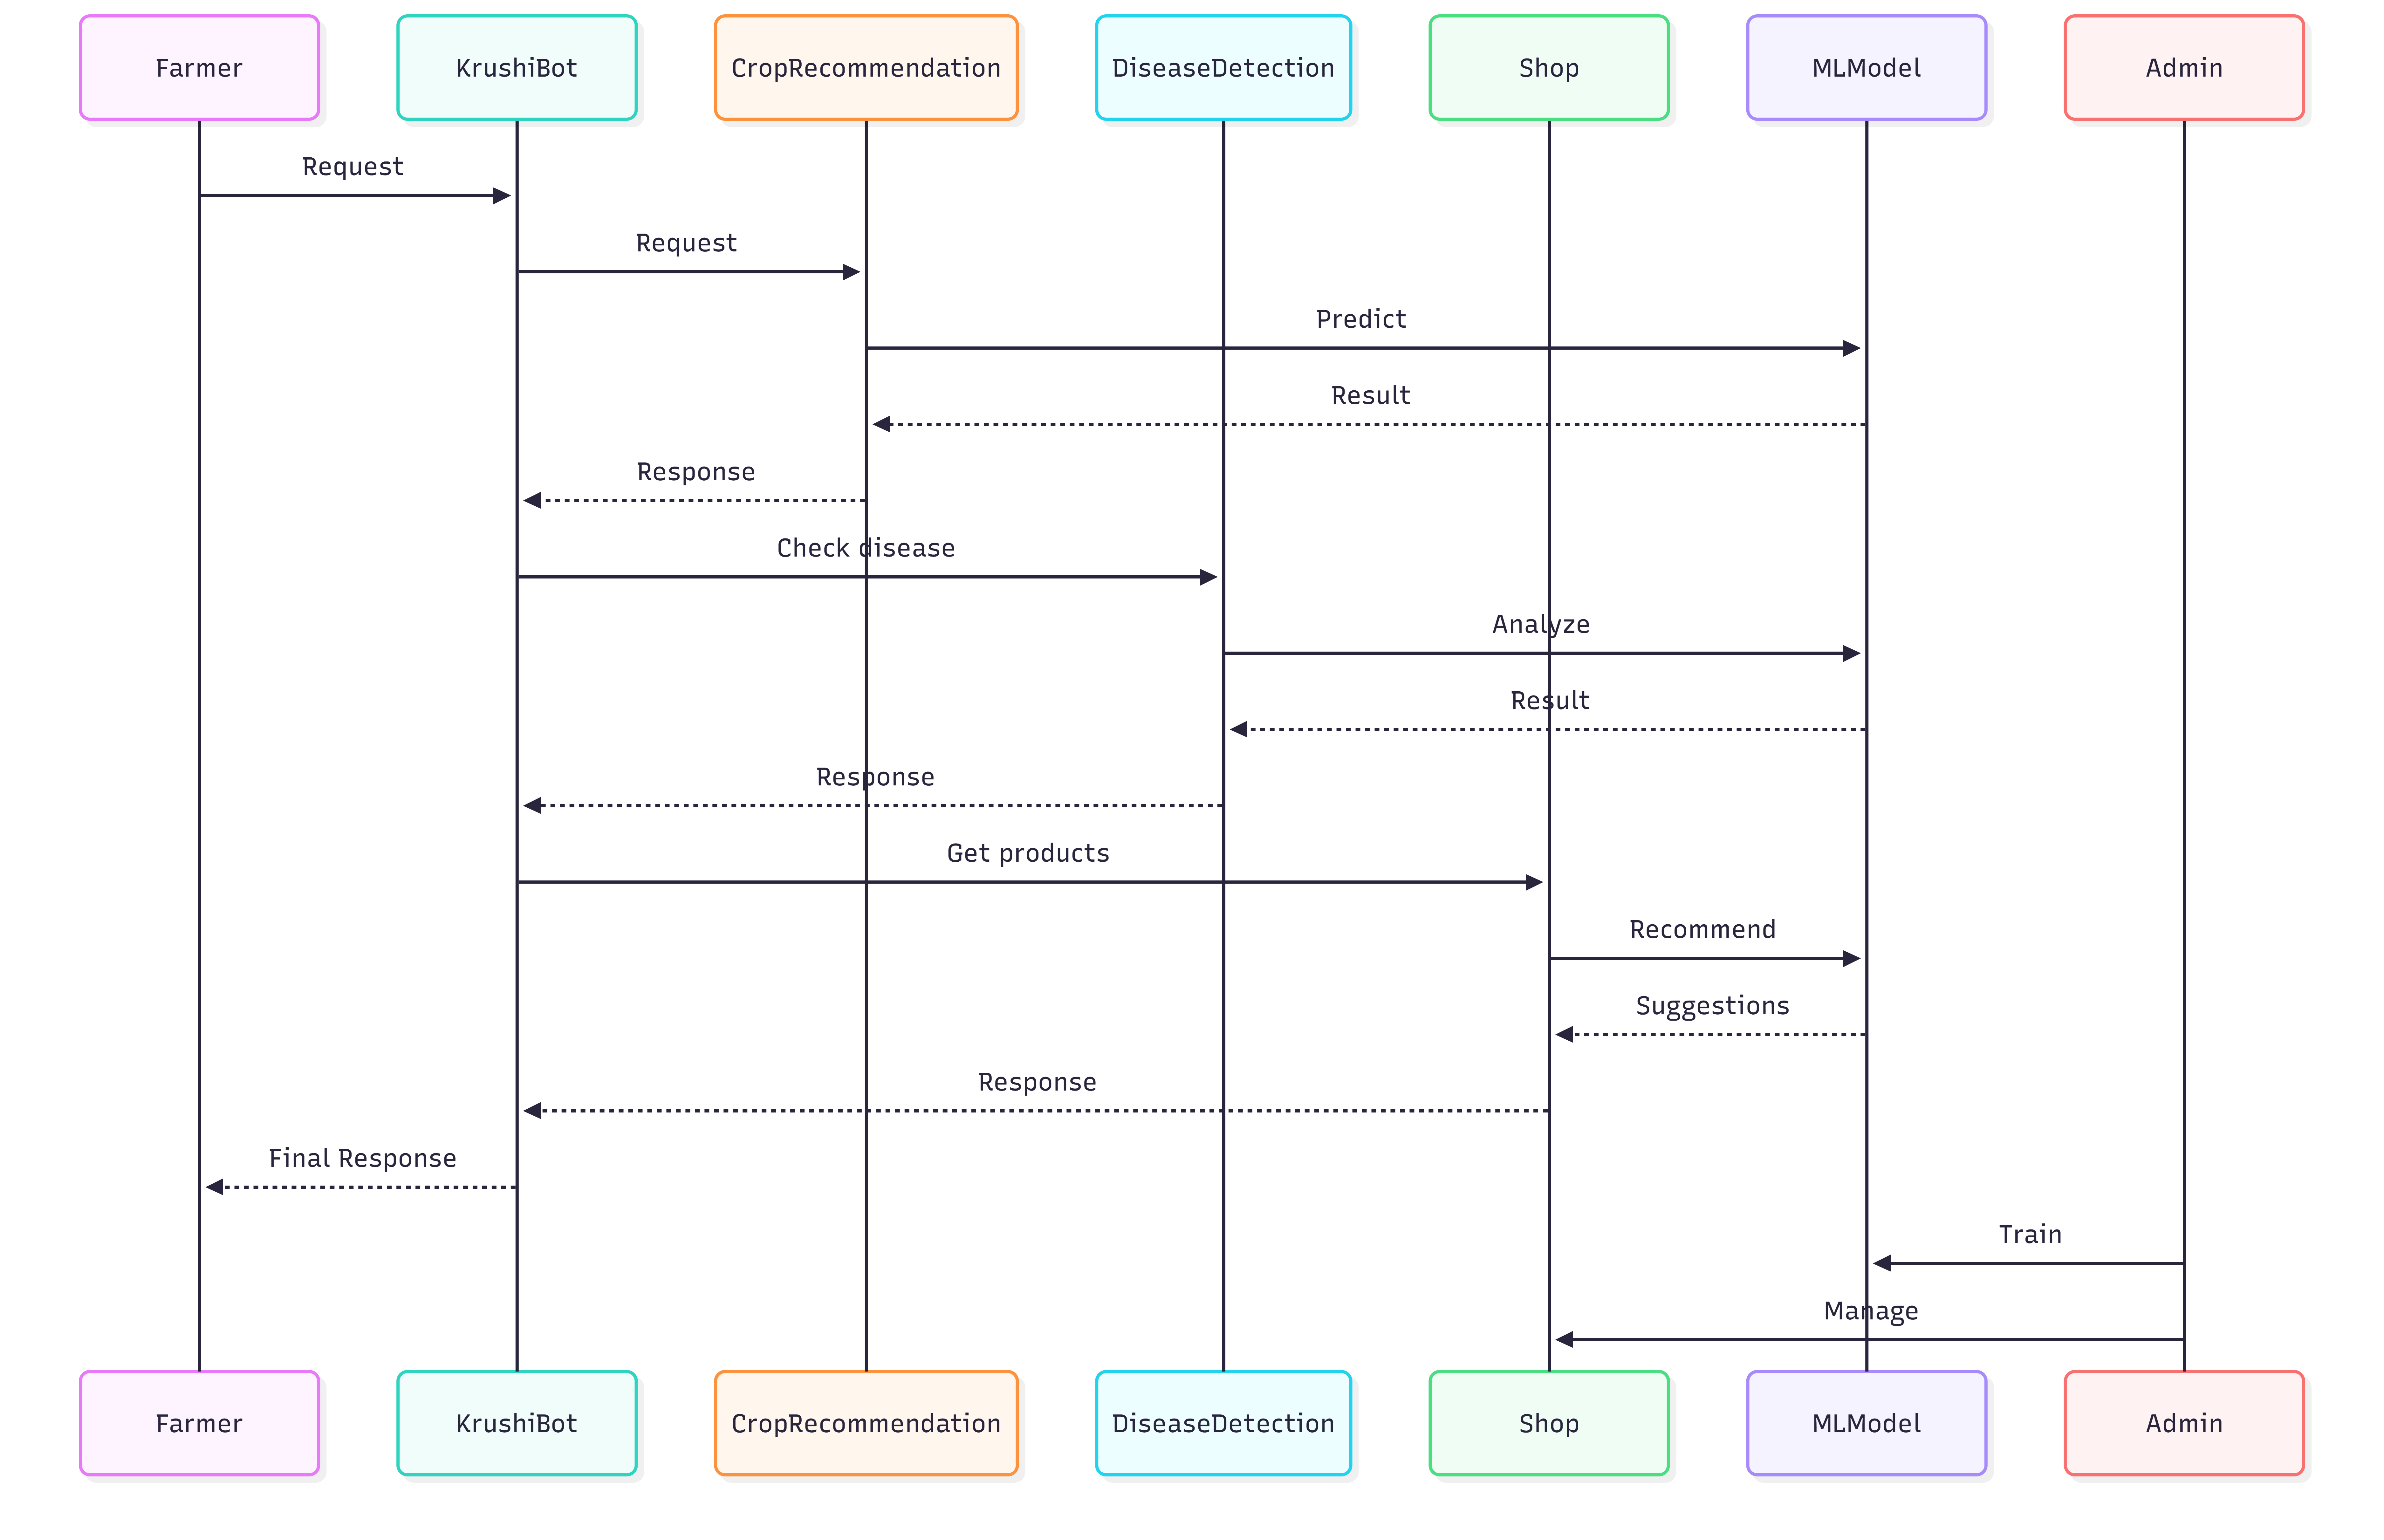
\includegraphics[scale=0.07]{project/images/image/sequence}
  \caption{Sequence Diagram}\label{Sequence Diagram}
\end{figure}

\newpage
  \item \textbf{Class Diagram}
   \begin{figure}[H]
 \centering
  % Requires \usepackage{graphicx}
 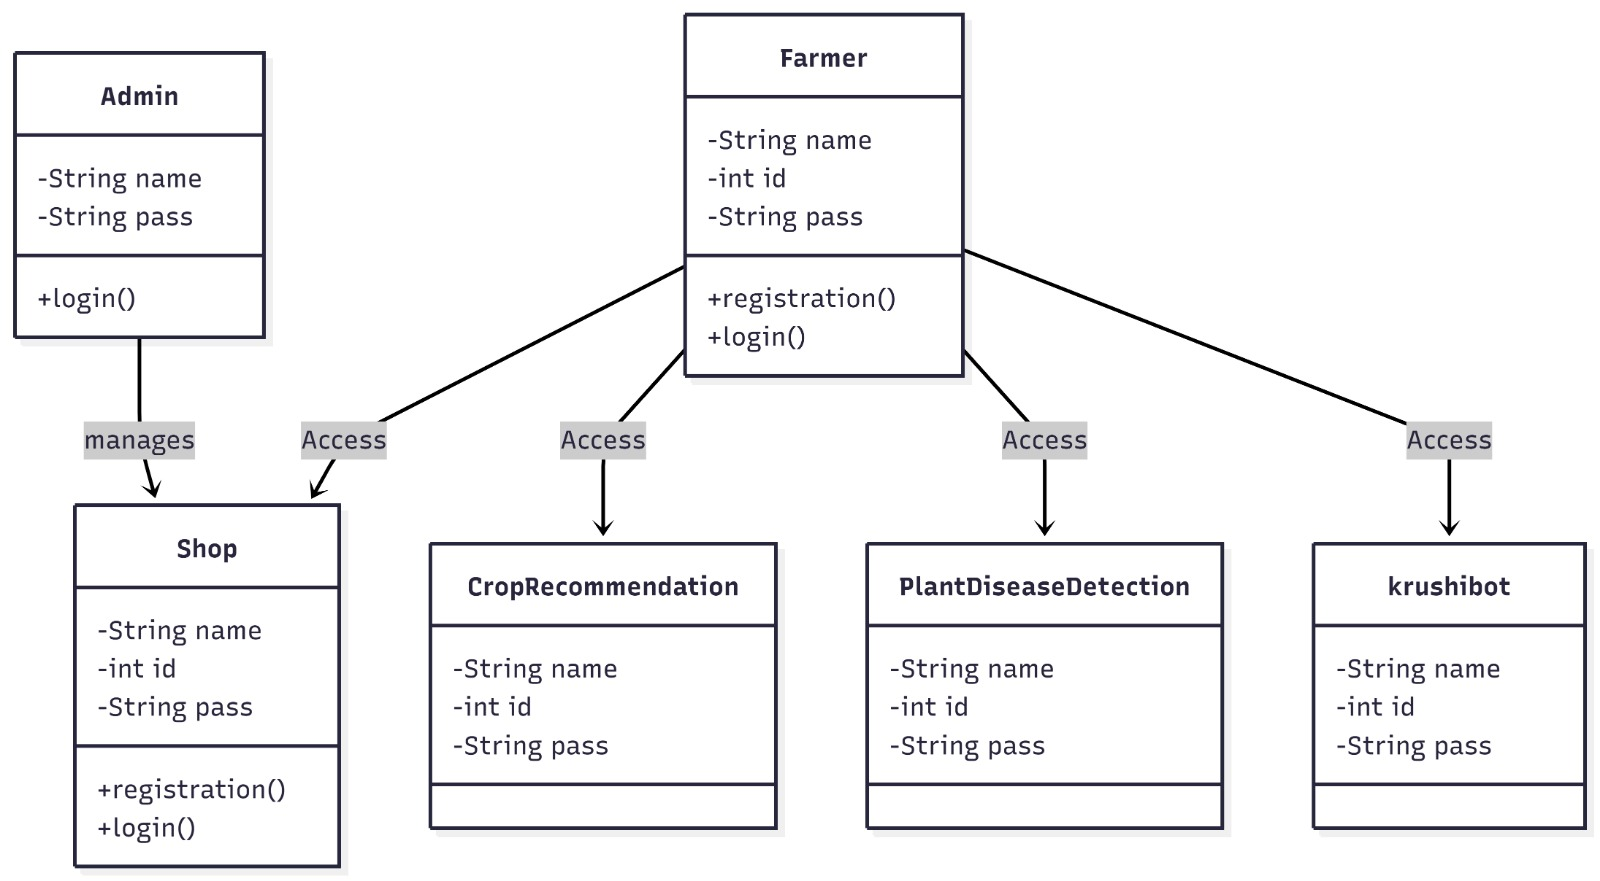
\includegraphics[scale=0.25]{project/images/image/class.jpeg}
  \caption{Class Diagram}\label{Class Diagram}
\end{figure}
\newpage
  \item \textbf{Activity Diagram}
\begin{figure}[H]
\centering
   % Requires \usepackage{graphicx}
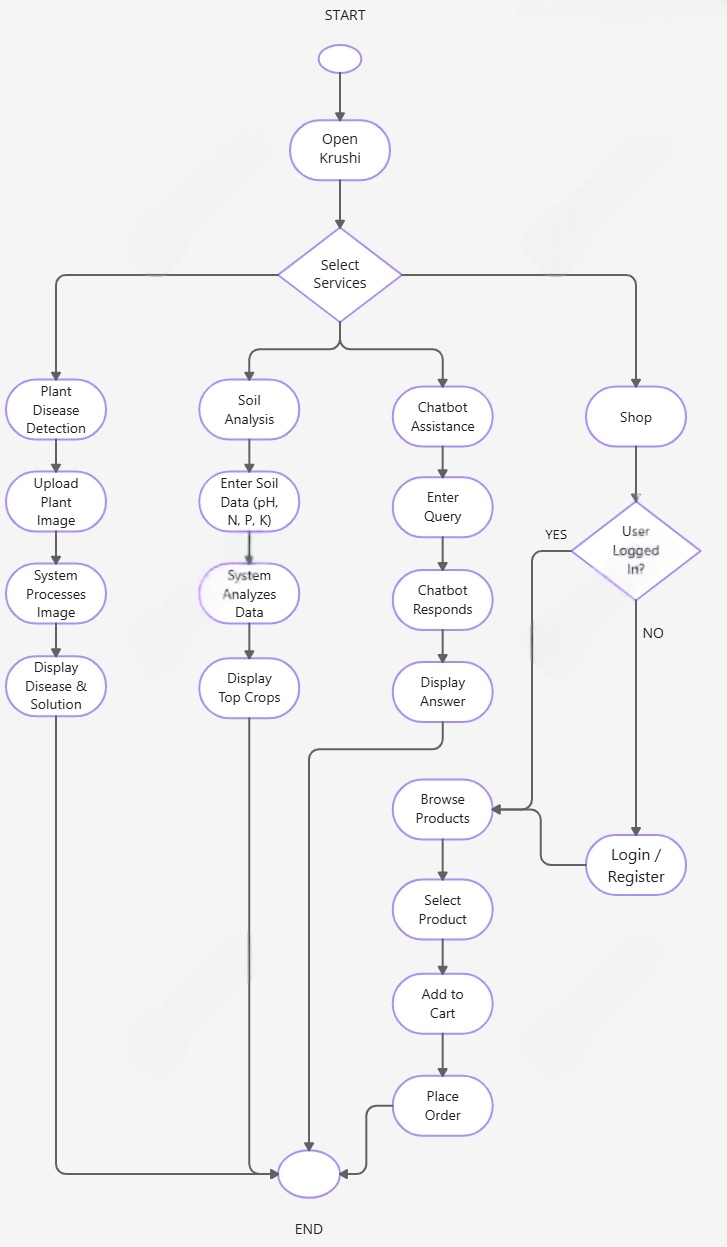
\includegraphics[scale=0.5]{project/images/image/user}
\caption{Activity Diagram for Farmer}\label{Activity Diagram}

\end{figure}
\end{enumerate}


 \chapter{Methodology}
 The development of the Krushi system will follow a systematic software development methodology
to ensure reliability, scalability, and usability.
\section{Requirement Analysis}
User and system requirements will be collected through discussions with farmers, mentors, and
domain experts. Functional requirements such as plant disease detection, soil analysis, chatbot
assistance, shop module, user registration, and payment handling will be identified. 
\section{Data Flow Diagram}
System architecture, database schema, and module interactions will be designed. Data Flow
Diagrams (DFDs), UML diagrams, and ER diagrams will be prepared to illustrate component relationships.
 \section{User Interface Design}
Responsive and user-friendly web pages will be designed using HTML, CSS, and JavaScript to
ensure easy accessibility for farmers. Multilingual and simple navigation interfaces will be
considered. 
\section{Backend Development}
Backend logic will be implemented using Django. Models, views, and controllers will be developed
for handling disease detection, soil analysis, chatbot response generation, product management and
order handling.
\section{ Machine Learning Integration}
The plant disease detection model will be integrated using pre-trained CNN architectures. Uploaded
images will be preprocessed and classified to generate disease predictions and suggestions. 
\section{Database Development}
PostgreSQL/SQLite databases will be designed to store user accounts, products, orders, chat history, soil records, and disease prediction logs. 
\section{API Development}
REST APIs using Django REST Framework will be implemented for mobile or web integration
supporting authentication, product services, disease prediction, soil analysis, and chatbot
communication. 
\section{Testing}
Unit testing, functional testing, usability testing, and security testing will be conducted to ensure
system stability. Errors and vulnerabilities will be identified and resolved. 
\section{Deployment}
The system will be deployed on a cloud platform or local server environment. Continuous
monitoring will ensure optimal performance. 
\section{Documentation}
User manuals and technical documentation will be prepared to support effective system maintenance
and user adoption.

\chapter{Implementation}
 This chapter includes the various stages of project in the form of Graphical user interface.
 \newline
 \enumerate

\item Main Home Page
\begin{center}
  % Requires \usepackage{graphicx}
  \begin{figure}[H]
  \centering
  
\includegraphics[scale=0.3]{project/images/image/home}
\caption{Home page of Our Web Application }
\label{fig:aLabelForReferencing}
  \end{figure}

\end{center}
\newpage
 \item Shop
\begin{center}
  % Requires \usepackage{graphicx}
  \begin{figure}[H]
  \centering
  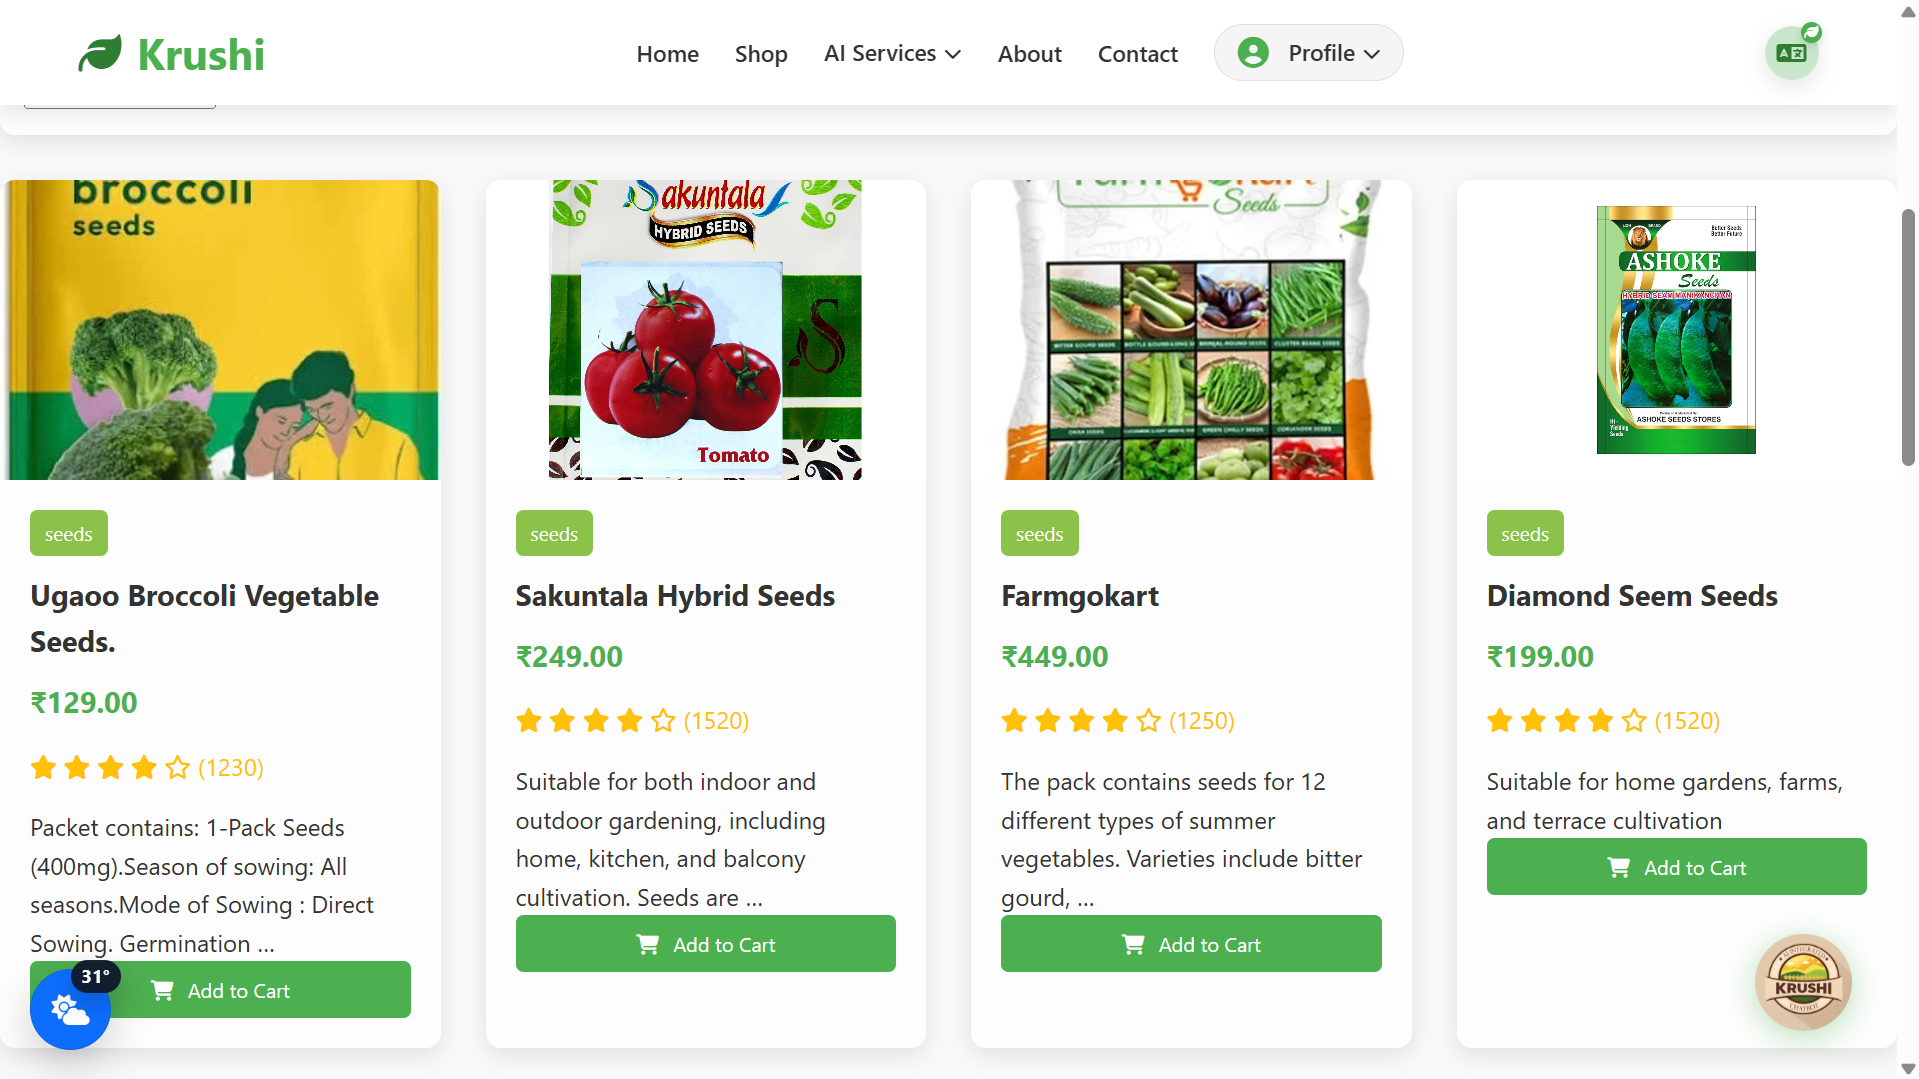
\includegraphics[scale=0.3]{project/images/image/shop.png}
\caption{Shop Page of Website. }
\label{fig:aLabelForReferencing}
  \end{figure}
\end{center}

\item Disease Detection
\begin{center}
  % Requires \usepackage{graphicx}
  \begin{figure}[H]
  \centering
  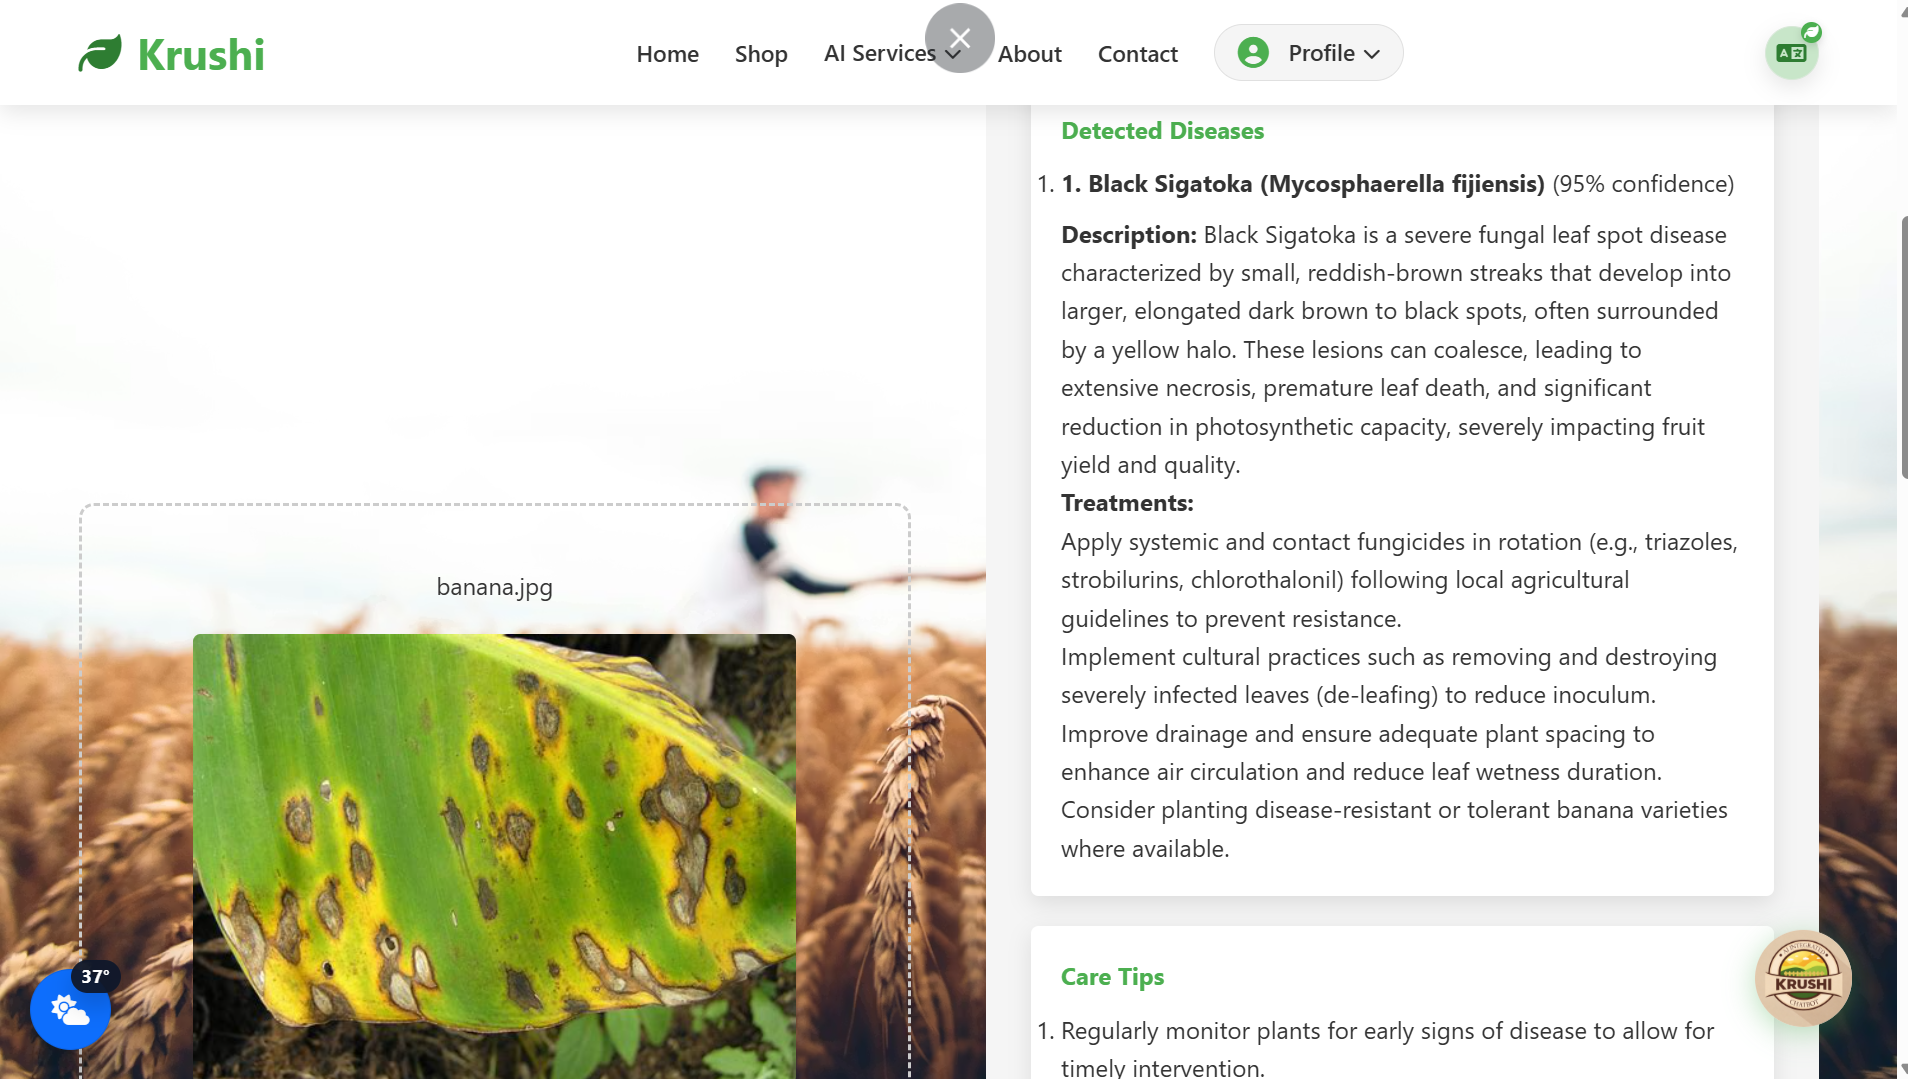
\includegraphics[scale=0.3]{project/images/image/disease-detection.png}
\caption{Disease Detection Page of Website. }
\label{fig:aLabelForReferencing}
  \end{figure}
\end{center}
\newpage

 \item Crop Recommendation
\begin{center}
  % Requires \usepackage{graphicx}
  \begin{figure}[H]
  \centering
  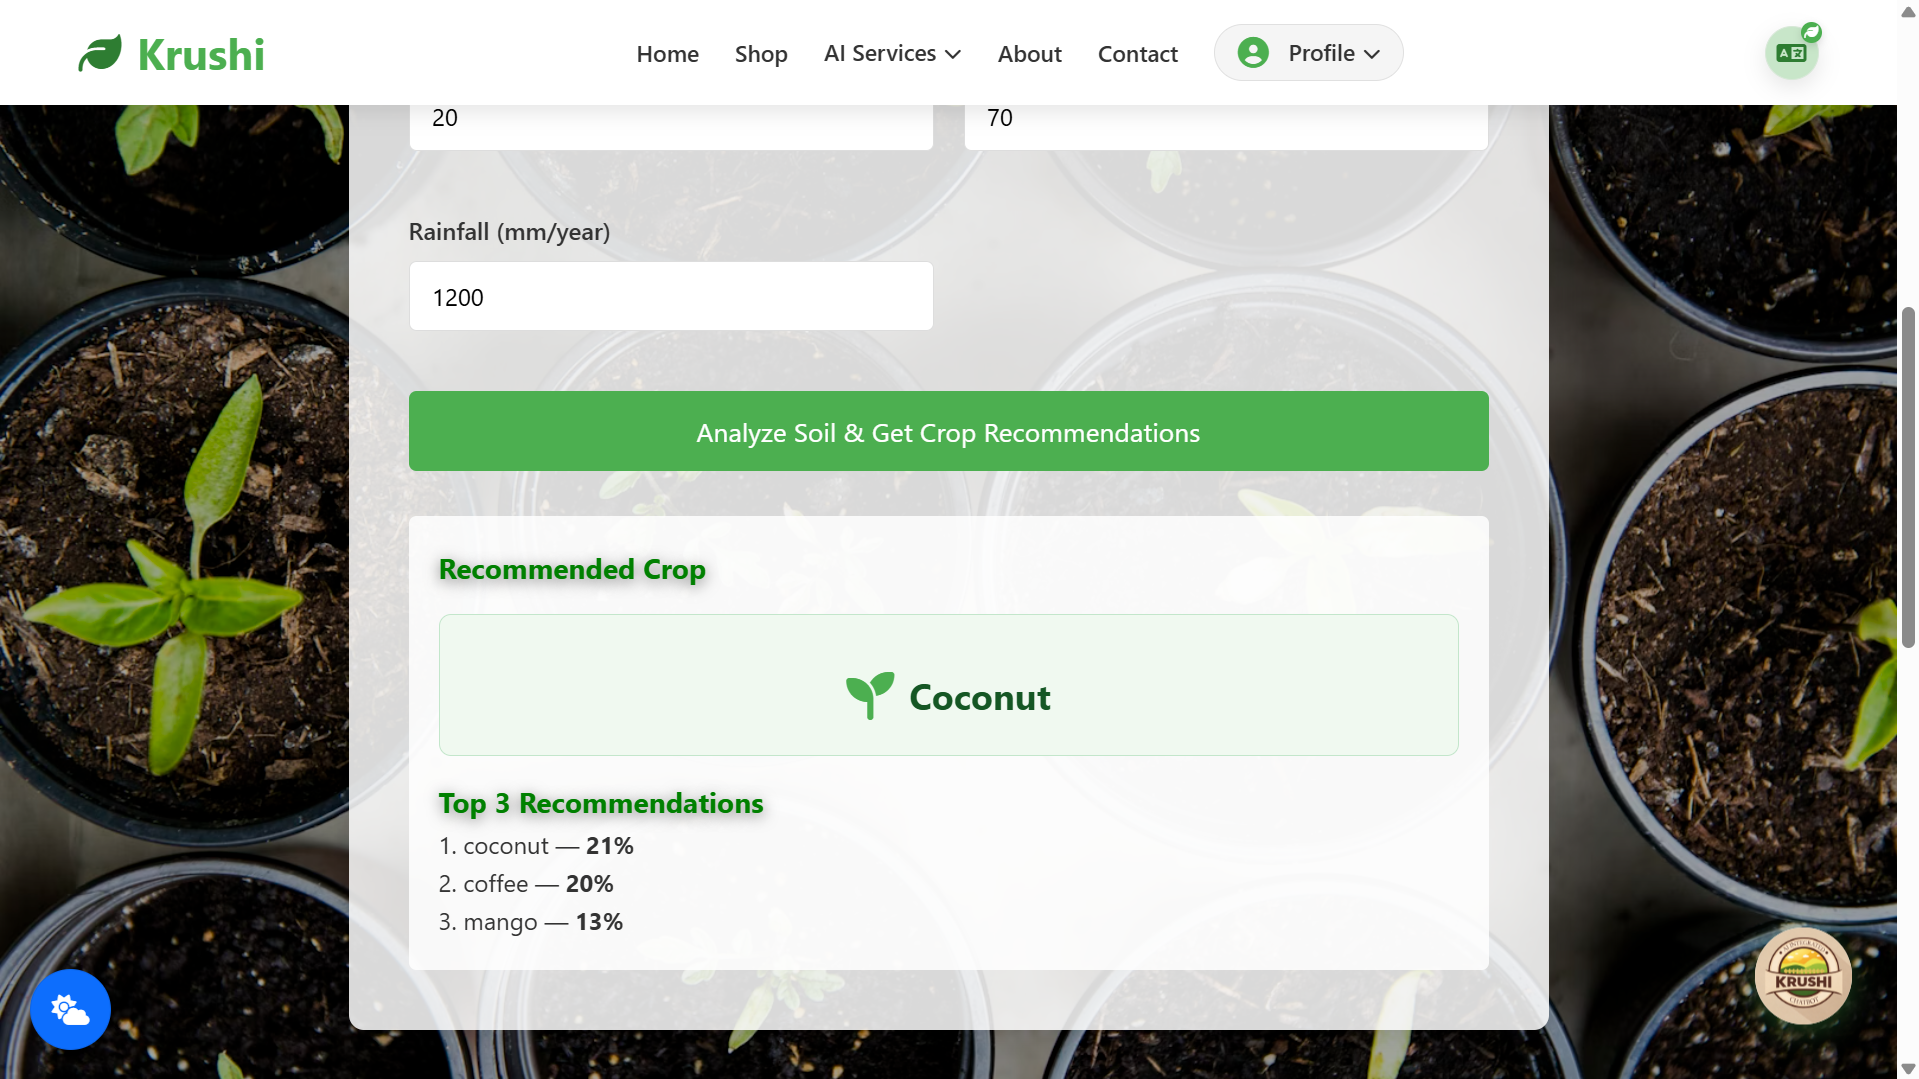
\includegraphics[scale=0.3]{project/images/image/crop-recommendation.png}
\caption{Crop Recommendation Page of Website. }
\label{fig:aLabelForReferencing}
  \end{figure}
\end{center}

\item Crop Planning
\begin{center}
  % Requires \usepackage{graphicx}
  \begin{figure}[H]
  \centering
  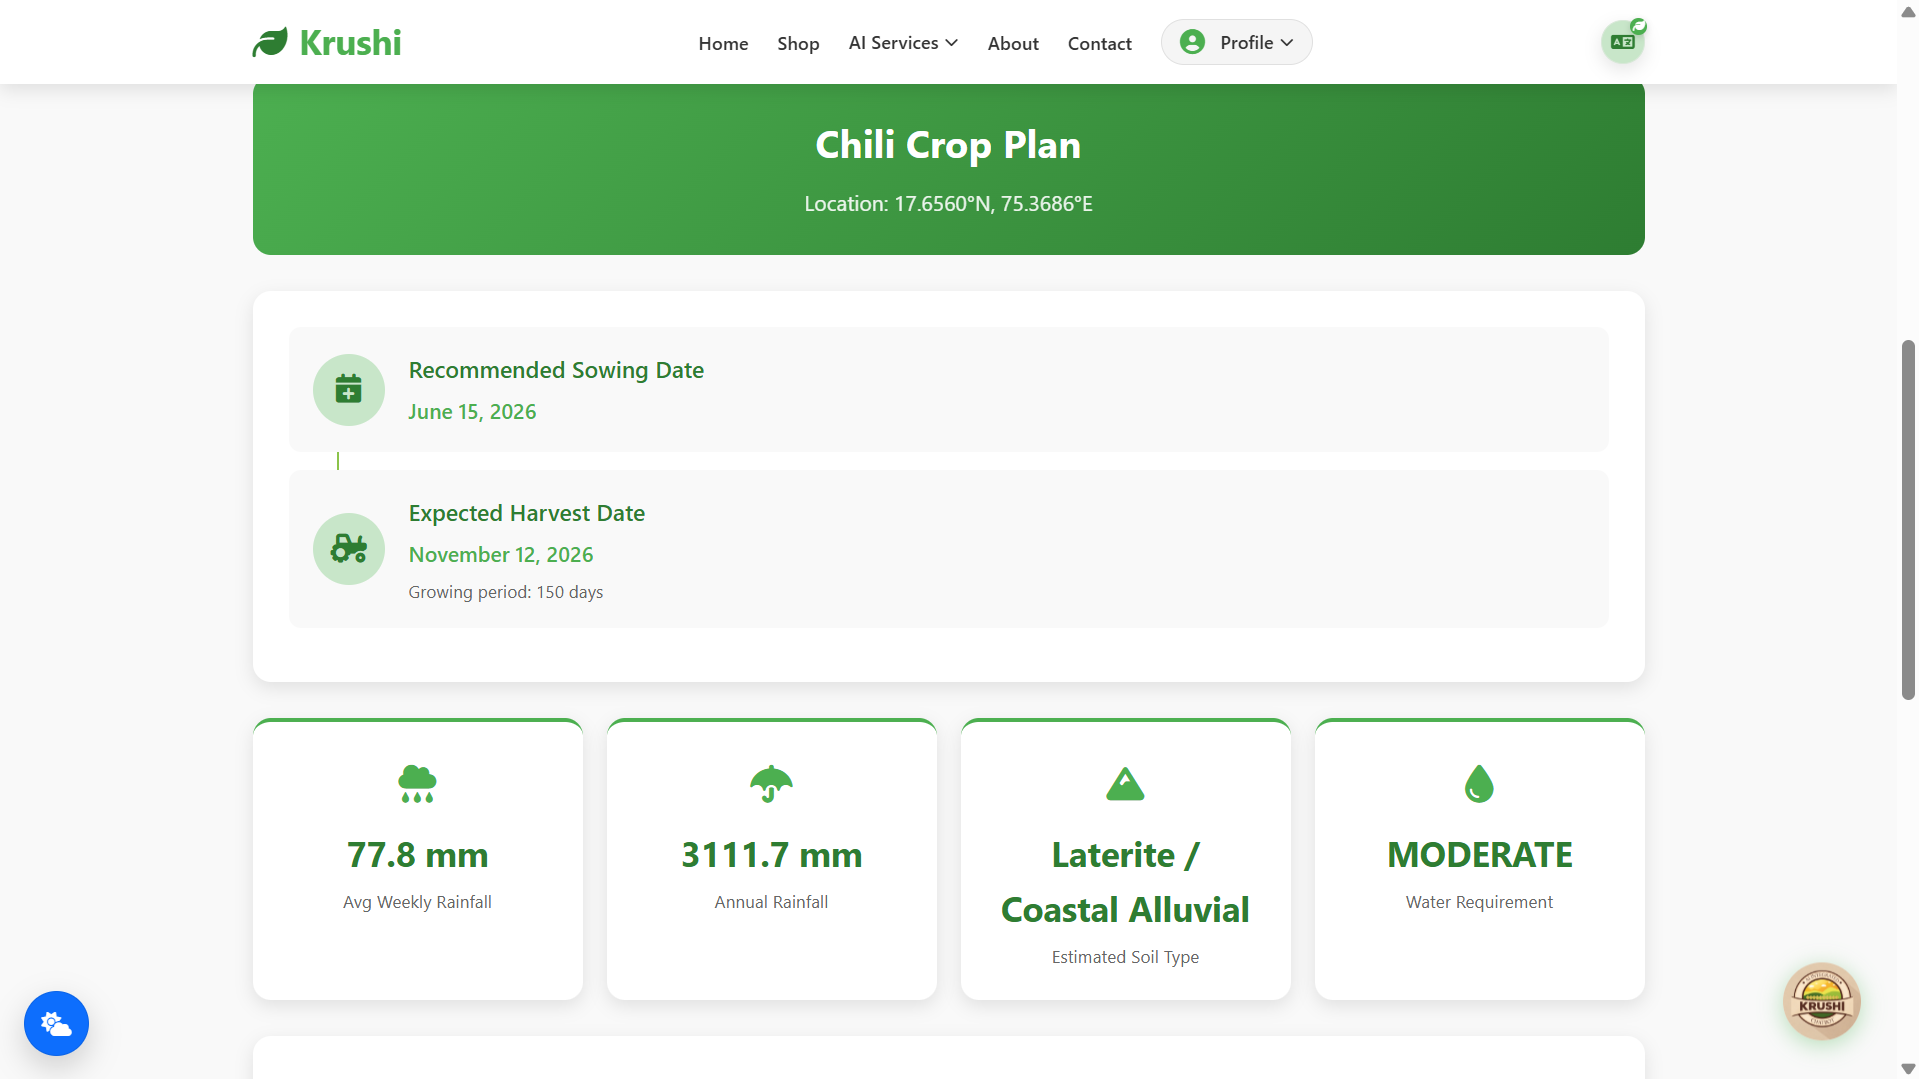
\includegraphics[scale=0.3]{project/images/image/crop-planning.png}
\caption{Crop Planning Page of Website. }
\label{fig:aLabelForReferencing}
  \end{figure}
\end{center}

 \item Chatbot
\begin{center}

  % Requires \usepackage{graphicx}
  \begin{figure}[H]
  \centering
  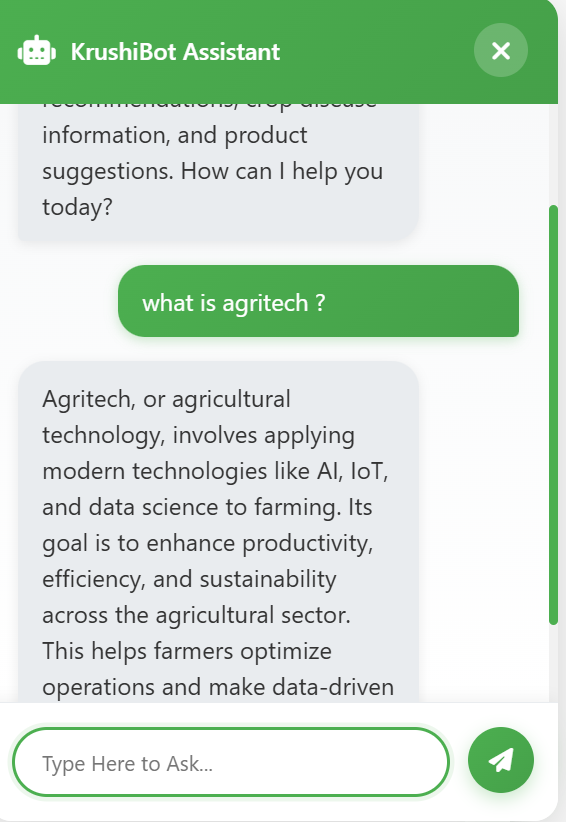
\includegraphics[scale=0.4]{project/images/image/chatbot.png}
\caption{Chatbot Page of Website. }
\label{fig:aLabelForReferencing}
  \end{figure}
\end{center}
 \item 7. Weather
\begin{center}

  % Requires \usepackage{graphicx}
  \begin{figure}[H]
  \centering
  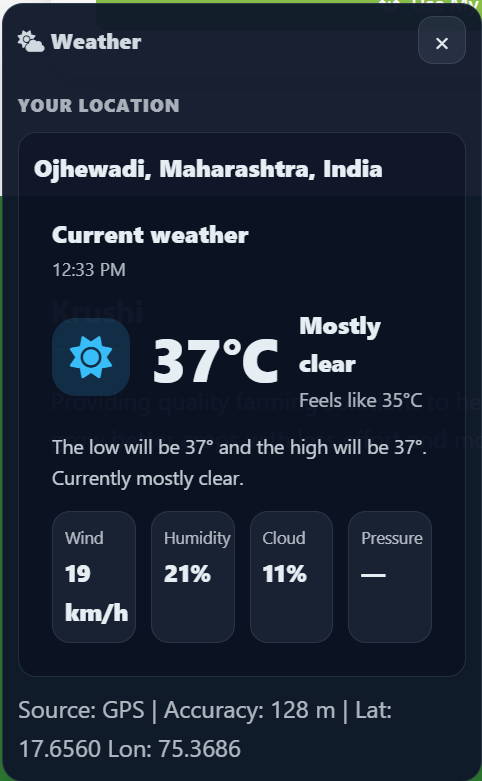
\includegraphics[scale=0.4]{project/images/image/weather.png}
\caption{Weather Page of Website. }
\label{fig:aLabelForReferencing}
  \end{figure}
\end{center}

 \endenumerate
